\large
	\def\imbcircle{(-210:2) circle (2.725cm)}
	\def\dscircle{(-330:2) circle (2.725cm)}
	\def\mdcircle{(-90:2) circle (2.725cm)}

	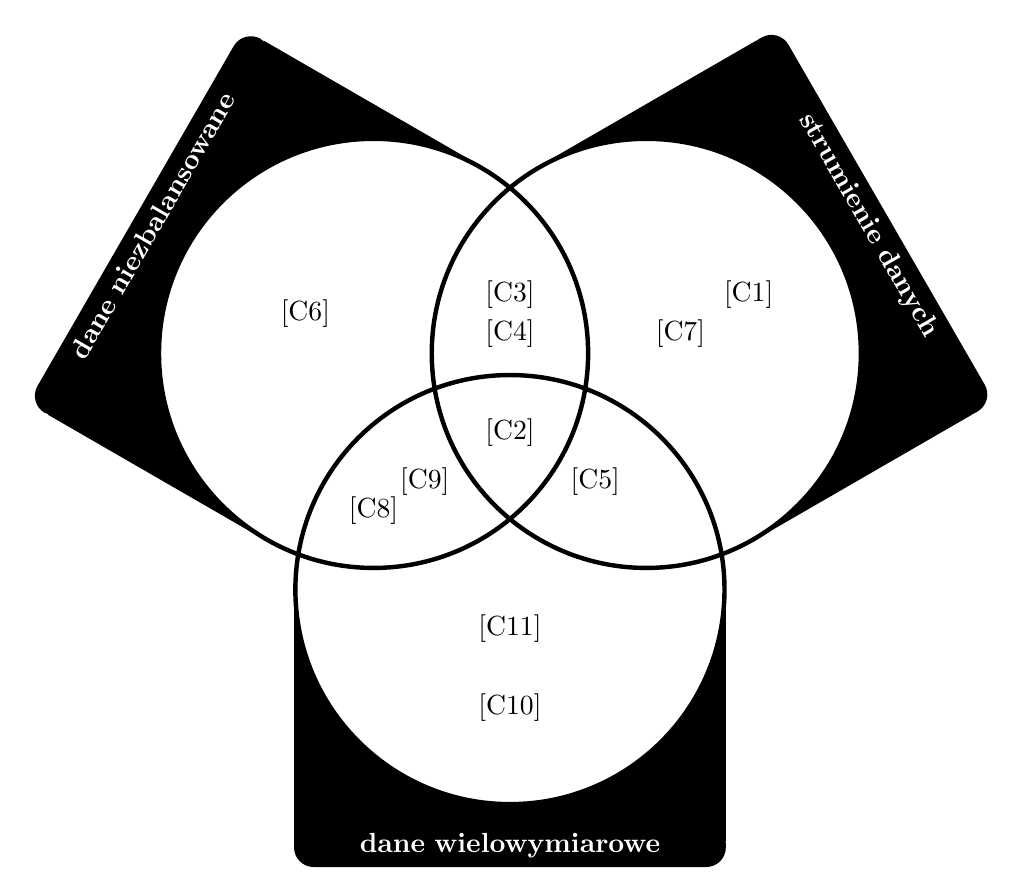
\begin{tikzpicture}
		%\draw[step=1.0,black,thin,dotted] (-5,-5) grid (5,5);
      	\begin{scope} % W miarę
    		%\clip \firstcircle;
    		%\fill[green!25] \mdcircle;
      	\end{scope}
      	\begin{scope} % W miarę
    		%\clip \firstcircle;
    		%\fill[yellow!25] \imbcircle;
      	\end{scope}
      	\begin{scope} % Git
    		%\clip \firstcircle;
    		%\fill[green!25] \dscircle;
      	\end{scope}
      	\begin{scope} % Problematyczny
    		%\clip \dscircle;
    		%\fill[red!25] \mdcircle;
      	\end{scope}
      	
      	\node[fill=black,rotate=-210-90, text width=5.25cm, text height=2.9cm] at (-210:3.625) {};
      	\node[fill=black,rotate=-330-90, text width=5.25cm, text height=2.9cm] at (-330:3.625) {};
      	\node[fill=black,rotate=0, text width=5.25cm, text height=2.9cm] at (-90:3.625) {};
      	
      	\node[color=white,fill=black,rotate=-210-90,rounded corners=.25cm, text width=5.25cm, align=center] at (-210:5.25) {\bfseries \textsc{dane niezbalansowane}};
      	\node[color=white,fill=black,rotate=-330-90,rounded corners=.25cm, text width=5.25cm, align=center] at (-330:5.25) {\bfseries \textsc{strumienie danych}};
		\node[color=white,fill=black,rotate=0,rounded corners=.25cm, text width=5.25cm, align=center] at (-90:5.25) {\bfseries \textsc{dane wielowymiarowe}};


    	\draw[fill=white] \imbcircle;
      	\draw[fill=white] \dscircle;
      	\draw[fill=white] \mdcircle;

      	
    	\draw[ultra thick] \imbcircle;
      	\draw[ultra thick] \dscircle;
      	\draw[ultra thick] \mdcircle;
      	

      	%\node[fill=white,rotate=-210-90,rounded corners=.25cm, text width=3cm, align=center] at (-210:4.5) {\bfseries Dane\\Niezbalansowane};
      	%\node[fill=white,rotate=-330-90,rounded corners=.25cm] at (-330:4.5) {\bfseries DS};
      	%\node[fill=white,rotate=-90+90,rounded corners=.25cm] at (-90:4.5) {\bfseries MD};
      	
      	% IMB
      	\node at (-210:3) {[C6]}; %7
      	
      	% IMB + DS
      	\node at (90:1.75) {[C3]};
      	\node at (90:1.25) {[C4]}; % 6
      	
      	% DS
      	\node at (-330:2.5) {[C7]};
      	\node at (-330:3.5) {[C1]};
      	
      	% MD
      	\node at (-90:2.5) {[C11]}; % 11
      	\node at (-90:3.5) {[C10]}; % 15
    
    	% IMB + MD
      	\node at (-330-180:1.25) {[C9]}; % 14
      	\node at (-330-180:2) {[C8]}; % 19
      	%\node at (-330-180:2.25) {[C10]}; % 19  	
      	
      	% DS + MD
      	\node at (-210-180:1.25) {[C5]};
      	
      	% ALL
      	\node at (0:0) {[C2]};
	\end{tikzpicture}